\documentclass[12pt,a4paper]{article}
%\usepackage{ctex}
\usepackage{amsmath,amscd,amsbsy,amssymb,latexsym,url,bm,amsthm}
\usepackage{epsfig,graphicx,subfigure}
\usepackage{enumitem,balance}
\usepackage{wrapfig}
\usepackage{mathrsfs,euscript}
\usepackage[usenames]{xcolor}
\usepackage[colorlinks,linkcolor = blue]{hyperref}
\usepackage[vlined,ruled,commentsnumbered,linesnumbered]{algorithm2e}

\newtheorem{theorem}{Theorem}
\newtheorem{lemma}[theorem]{Lemma}
\newtheorem{proposition}[theorem]{Proposition}
\newtheorem{corollary}[theorem]{Corollary}
\newtheorem{exercise}{Exercise}
\newtheorem*{solution}{Solution}
\newtheorem{definition}{Definition}
\theoremstyle{definition}
\usepackage{listings}


%
\definecolor{mygreen}{rgb}{0,0.6,0}
\definecolor{mygray}{rgb}{0.5,0.5,0.5}
\definecolor{mymauve}{rgb}{0.58,0,0.82}
\lstset{
	backgroundcolor=\color{white}, 
	basicstyle = \footnotesize,       
	breakatwhitespace = false,        
	breaklines = true,                 
	captionpos = b,                    
	commentstyle = \color{mygreen}\bfseries,
	extendedchars = false,             
	frame =shadowbox, 
	framerule=0.5pt,
	keepspaces=true,
	keywordstyle=\color{blue}\bfseries, % keyword style
	language = C++,                     % the language of code
	otherkeywords={string}, 
	numbers=left, 
	numbersep=5pt,
	numberstyle=\tiny\color{mygray},
	rulecolor=\color{black},         
	showspaces=false,  
	showstringspaces=false, 
	showtabs=false,    
	stepnumber=1,         
	stringstyle=\color{mymauve},        % string literal style
	tabsize=2,          
	title=\lstname                      
}

%\numberwithin{equation}{section}
%\numberwithin{figure}{section}

\renewcommand{\thefootnote}{\fnsymbol{footnote}}

\newcommand{\postscript}[2]
 {\setlength{\epsfxsize}{#2\hsize}
  \centerline{\epsfbox{#1}}}

\renewcommand{\baselinestretch}{1.0}

\setlength{\oddsidemargin}{-0.365in}
\setlength{\evensidemargin}{-0.365in}
\setlength{\topmargin}{-0.3in}
\setlength{\headheight}{0in}
\setlength{\headsep}{0in}
\setlength{\textheight}{10.1in}
\setlength{\textwidth}{7in}
\makeatletter \renewenvironment{proof}[1][Proof] {\par\pushQED{\qed}\normalfont\topsep6\p@\@plus6\p@\relax\trivlist\item[\hskip\labelsep\bfseries#1\@addpunct{.}]\ignorespaces}{\popQED\endtrivlist\@endpefalse} \makeatother
\makeatletter
\renewenvironment{solution}[1][Solution] {\par\pushQED{\qed}\normalfont\topsep6\p@\@plus6\p@\relax\trivlist\item[\hskip\labelsep\bfseries#1\@addpunct{.}]\ignorespaces}{\popQED\endtrivlist\@endpefalse} \makeatother



\begin{document}
\noindent

%========================================================================
\noindent\framebox[\linewidth]{\shortstack[c]{
\Large{\textbf{Lab03 Sorting and Selection}}\vspace{1mm}\\
VE281 - Data Structures and Algorithms, Xiaofeng Gao, Autumn 2019}}
%VE281 - Data Structures and Algorithms, Xiaofeng Gao, Autumn 2019}}
\begin{center}
	\footnotesize{\color{blue}$*$ Name:Jin Zhejian	\quad Student ID: 517370910167 \quad Email: jinzhejian@outlook.com}
\end{center}




%\section{Motivation}
%\begin{enumerate}
%    \item To give you experience in implementing various sorting algorithms and two linear-time selection algorithms, i.e., random and deterministic selection algorithms.
%    \item To empirically study the run time efficiency of the sort algorithms and two selection algorithms and compare the run time efficiency of the selection algorithms with the sorting algorithms.
%\end{enumerate}
\section{Preparation}
 In order to show the relationship between runtime and array size better, I choose the array size 100, 500, 1000, 5000, 10000, 50000. I  generate random numbers and put them in the array, and then save them in 6 .txt file. The source code is shown below.
 \begin{lstlisting}[caption={generate.cpp}]
#include <iostream>
#include <fstream>
#include <stdlib.h>
using namespace std;

int main(){
	fstream fso("data_50000.txt", ios::out);
	int size = 50000;
	int i;
	for(i = 0; i < size; ++i)
	fso << rand() << ' ';
	fso.close();

	fstream fsi("data_50000.txt", ios::in);
	int x[size];
	for(i = 0; i < size; ++i)
	fsi >> x[i];

	int j;
	for(i = 0; i < size; ++i)
		for(j = size-1; j > i; --j)
			if(x[j - 1] > x[j]){
			int t = x[j];
			x[j] = x[j - 1];
			x[j - 1] = t;
			}
	for(i = 0; i < size; ++i)
		cout << x[i] << '\t';
}
 \end{lstlisting}

In order to calculate the runtime of my realization more precisely, I do 20 times of the sort and calculate the average runtime. Also, for the selection algorithm, I choorse 20 different i numbers and calculate the average runtime.

\newpage
\section{Sort algorithms}

In this lab, I studied 5 sort algorithms, they are: BubbleSort ,InsertionSort,SelectionSort   MergeSort, and QuickSort. I chose the array size 100, 500, 1000, 5000, 10000, 50000, and I record each of the run times of the five sort algoritms.
 
The graph and my data are shown as follows:
\begin{figure}[ht]
	\centering
	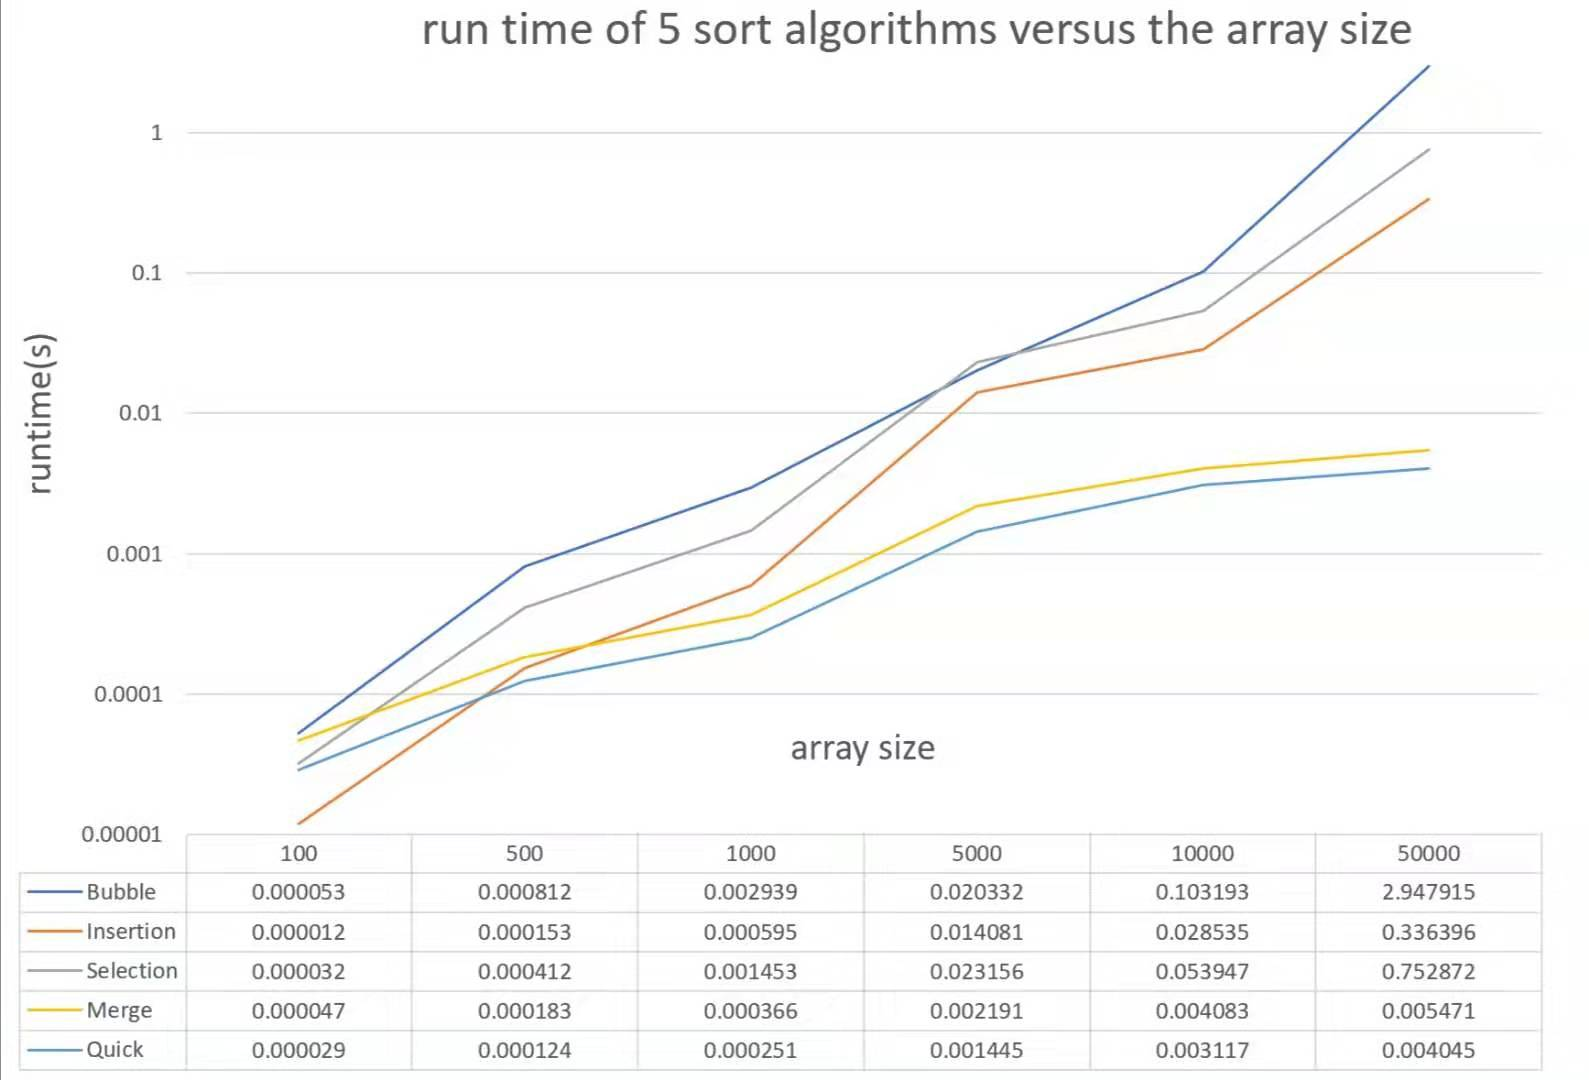
\includegraphics[scale=0.32]{Lab03_1.jpg}
	\caption{runtime of 5 sort algorithms versus the array size}
\end{figure}

From the figure, we can find that the runtime of Merge Sort and Quick Sort is faster that of Bubble Sort, Insertion Sort, and Selection Sort.  

In my realization, the Insertion Sort is several times faster than the Bubble Sort. One potential reason is that, in my code, in the while loop of Bubble Sort, the program need additionally to judge whether the Boolean variable sorted is true or false, which causes additional runtime.  Of course, the Bubble Sort of my realization can be improved. Only needs to uncomment the commented part \textbf{if (sorted)\{break;\}}. The runtime will be fasten observably.



For Merge Sort and Quick Sort, we can see from the figure that the two algorithms have the same time complexity, and  Merge Sort is a little slower than the Quicksort. From my guess, the difference is due to the reason that Merge Sort uses Dynamic Memory in the heap, which is slower than the stack operations. This will be discussed further in the Selection algorithms part.

\newpage
\section{Selection algorithms}

In this part, I compare the runtime of the two selection algorithms( random selection algorithm and deterministic selection algorithm) with the quick sort algorithm. The second figure indicates the runtime of 2 different selection algorithms and quick sort versus the array size, which is shown as follows:

\begin{figure}[ht]
	\centering
	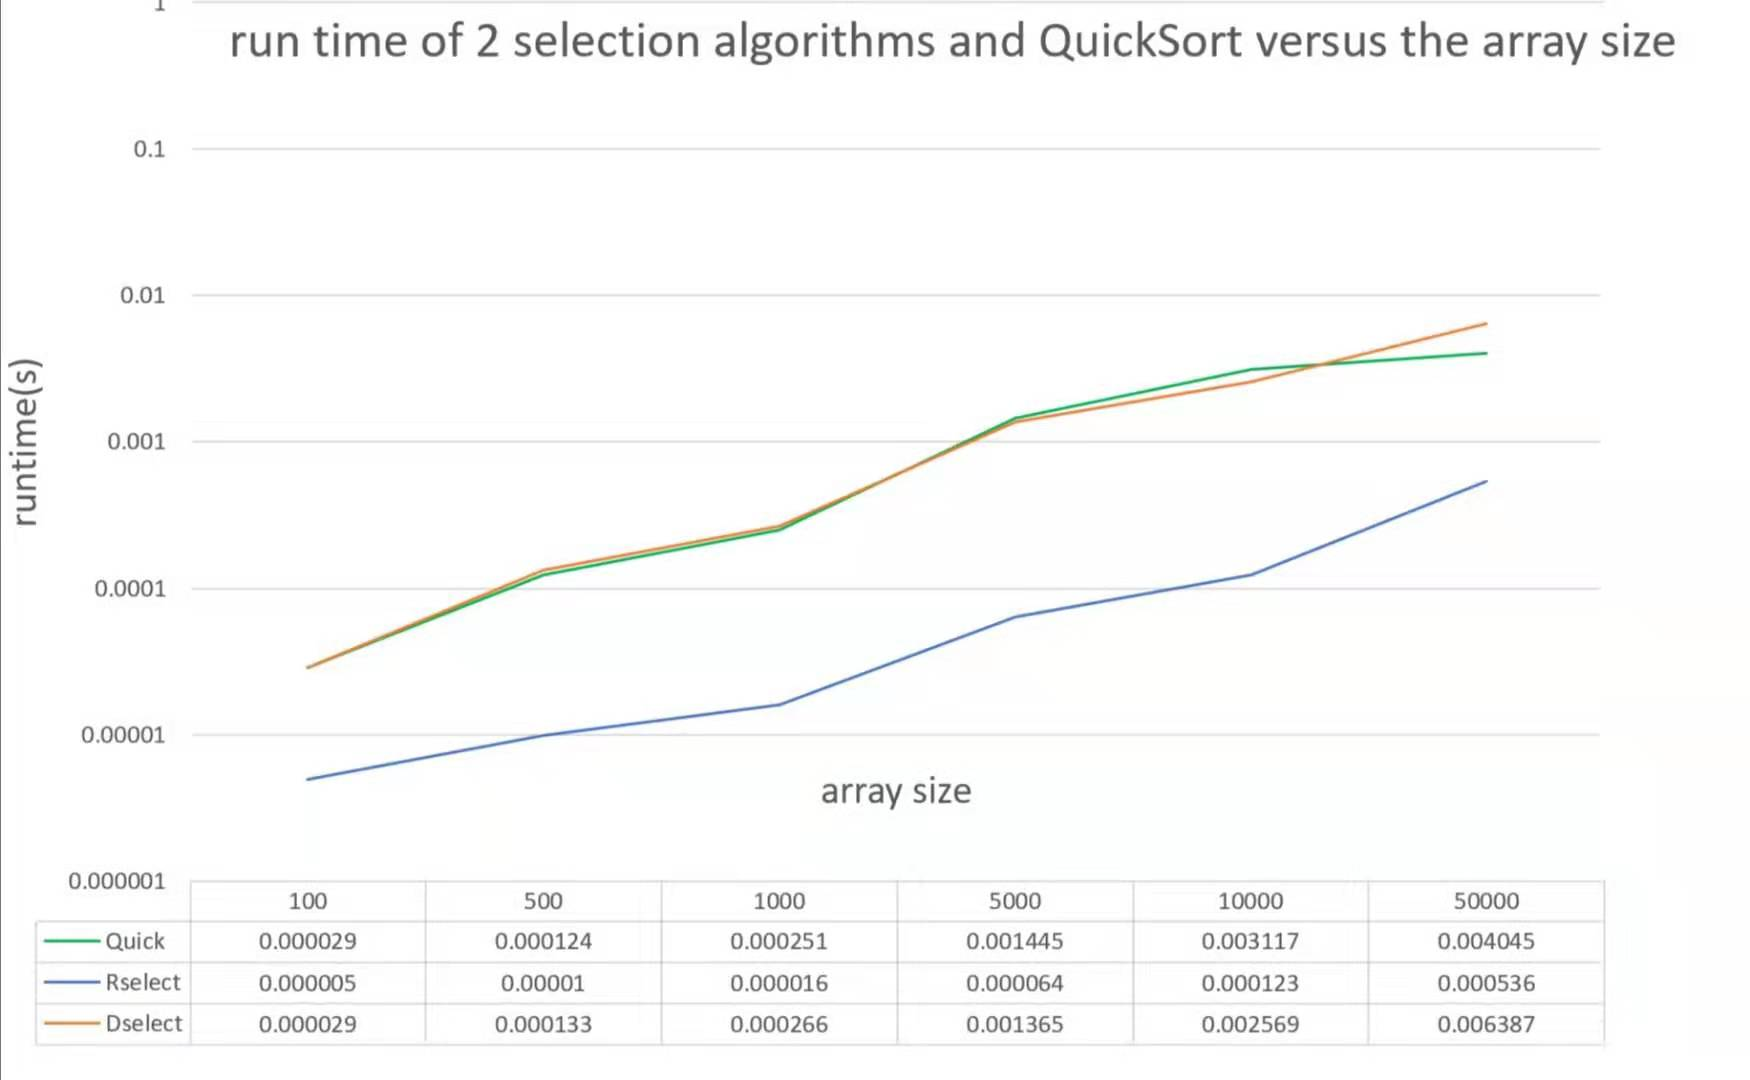
\includegraphics[scale=0.3]{Lab03_2.jpg}
	\caption{runtime of 2 selection algorithms and QuickSort versus the array size}
\end{figure}

The result does not satisfy our theoretical knowledge, although the graph shows the three algorithms have the same growing speed. Deterministic Selection is a faster version of Random Selection theoretically, however, in my realization, the Dselect is much faster than R select. My expatiation is that: Dselect and Quick Sort use\textbf{ Dynamic Memory}, such as \textbf{int *C = new  int[size]} in Dselect. It is done in the heap in the memory, whose memory management speed is slower than the stack, because it needs to dynamically allocate the memory when running the code. 


\end{document}
